\documentclass[]{beamer}
\usetheme{Dresden}
% \useoutertheme{split}

\usepackage{color}
\usepackage{graphicx}
\usepackage{listings}
\usepackage{lmodern} %% allow bold keywords
\usepackage{menukeys}
\usepackage{qtree}

\definecolor{darkgreen}{rgb}{0,0.5,0}
\definecolor{lightblue}{rgb}{0.2,0.2,1}

\lstset{language=Java,
	basicstyle=\ttfamily\footnotesize,
	keywordstyle=\color{purple},
	commentstyle=\color{darkgreen},
	numberstyle=\tiny\color{gray},
	stringstyle=\color{blue},
	tabsize=4,
	showstringspaces=false,
	breaklines=true,
	keepspaces=true,
	numbers=left,
	escapechar=@
}

\title{Java 07}
\subtitle{Debugging}
\author{FSR Informatik}
\date{\today}

\begin{document}

\begin{frame}
\titlepage
\end{frame}
\begin{frame}{Overview}
\tableofcontents
\end{frame}

\section{Debugging}
\subsection{Overview}
\begin{frame}{}
	A debugger helps the programmer to trace errors in their code.
	\vfill
	Normally a program executes every line of code and stops afterwards.
	With a debugger you can watch every state of the execution.\\
	
	The inspection of a specific state can help to find errors.
\end{frame}

\subsection{Breakpoints}
\begin{frame}{Debug Perspective}
	Eclipse offers multiple perspectives for multiple tasks.
	\begin{itemize}
		\item The \emph{Java perspective} is standard while programming.
		\item The \emph{Debug perspective} can be used for debugging.
	\end{itemize}
	\vfill
	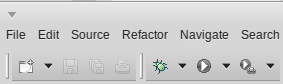
\includegraphics[width=10em]{res/debug_start.png} \\
	The bug icon starts the debugger. You can also press \keys{F11}.
	\vfill
	You can change the perspective via:
	\menu[,]{Window, Open Perspective, ...} \\
	or press \keys{CTRL + F8}.
\end{frame}

\begin{frame}{Breakpoint}
	A breakpoint marks a specific line in the code.
	\vfill
	While debugging the excecution of the program will stop before every marked line.
	At this point you see every current variable and object with their current values.
	\vfill
	The debugger steps through the code breakpoint by breakpoint.
\end{frame}

\begin{frame}{Toggle Breakpoints}
	With \keys{Shift + Ctrl + B} you can add or remove a breakpoint to the current line.
	\vfill
	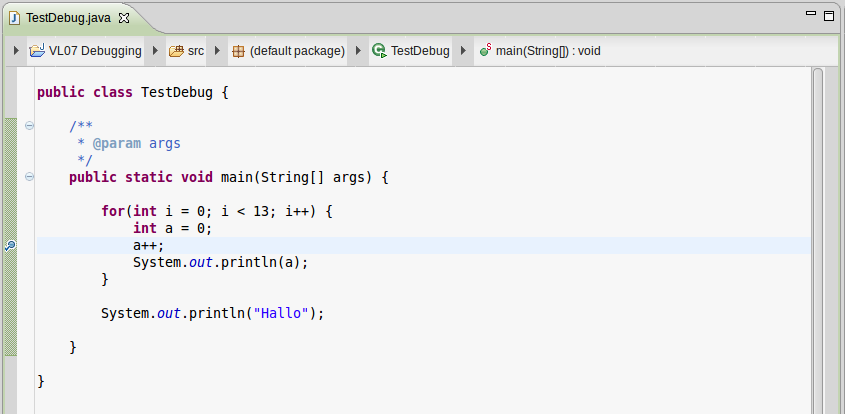
\includegraphics[width=25em]{res/debug_breakpoint.png} \\
	Breakpoint at the line: \texttt{a++;}
\end{frame}

\begin{frame}[fragile]{Stepping through the Code - 1}
	If your code contains breakpoints Eclipse will jump to the \emph{Debug Perspective} automatically
	when you start the debugger.
	\begin{lstlisting}
	public class TestDebug {

	    public static void main(String[] args) {
		
	        for(int i = 0; i < 13; i++) {
	            int a = 0;
	            a++;
	            System.out.println(a);
	        }
	    }
	}
	\end{lstlisting}
	Assume breakpoints in line 6, 7 and 8. Start the debugger.
\end{frame}

\begin{frame}{Stepping through the Code - 2}
	The table with all current variables is in the upper right corner.
	The view is called \emph{Variables}.
	\vfill
	You can step through the code with \keys{F8} or using the green arrow symbol. 
	The red square or \keys{Ctrl + F2} will end the debugging.\\
	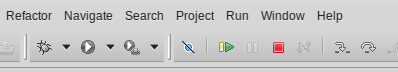
\includegraphics[width=15em]{res/debug_step.png} \\
	\vfill
	While stepping through the code variables appear and change their values.
	Current changes of the values will be marked yellow.
\end{frame}

\subsection{Stack Trace}
\begin{frame}[fragile]{Stack}
	The stack trace shows all methods a program called at a certain point.
	\vfill
	Every method call increases the stack. \\
	Every return and end of a void-method decreases the stack.
\end{frame}

\begin{frame}[fragile]{Development over Time}
	\begin{lstlisting}[basicstyle=\ttfamily\scriptsize, firstnumber = 1]
	public static void a() {
	    c();
	}
	public static void b() {}
	public static void c() {
	    b();
	}
	public static void main (String[] args) {
	    a();
	    b();
	}
	\end{lstlisting}
	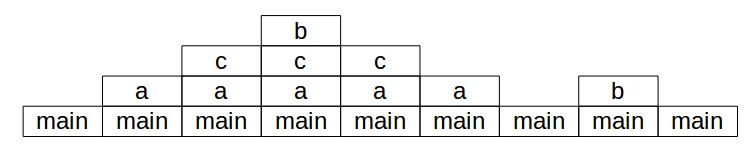
\includegraphics[width=25em]{res/debug_stack.png} \\
\end{frame}

\begin{frame}[fragile]{Printed Stack Trace}
	\begin{lstlisting}[basicstyle=\ttfamily\scriptsize, firstnumber = 3]
	public static void a() {
	    c();
	}
	public static void b() {
	    throw new RuntimeException();
	}
	public static void c() {
	    b();
	}
	public static void main (String[] args) {
	    a();
	    b();
	}
	\end{lstlisting}
	\footnotesize\texttt{	
	Exception in thread "main" java.lang.RuntimeException\\
	at TestStack.b(TestStack.java:8)\\
	at TestStack.c(TestStack.java:12)\\
	at TestStack.a(TestStack.java:4)\\
	at TestStack.main(TestStack.java:16)}
\end{frame}

\begin{frame}{Debug Perspective}
	The view \emph{Debug} shows the current stack. \\
	It is located in the upper left corner of the debug perspective.
\end{frame}

\end{document}